\documentclass[pdftex,10px,a4paper,oneside]{article}

\usepackage[utf8]{inputenc}
\usepackage{graphicx}
\usepackage{lipsum}
\usepackage{fancyhdr}
\usepackage{setspace}
\usepackage[hyphens]{url}
\usepackage{listings}


\title{Comparing Scikit-learn Classifiers with Local Feature Selector Classifier}
\author{Chukwuebuka Amaefula }
\date{August 2020}
\begin{document}
\maketitle
\begin{spacing}{2}
    \vspace{20mm}
    \begin{center}
        \textbf{\large Department of Computer Science}\\
        {\large Memorial University of Newfoundland}\\
    \end{center}
\end{spacing}
\clearpage
\section{Datasource}
Given samples of two species of Iris (Iris setosa, Iris virginica) I will compare the binary classification performance of three scikit-learn classifier and third party classification algorithms:
\begin{itemize}
  \item K-Nearest Neighbor
  \item Gaussian Bayes
  \item Decision Tree
  \item Local Feature Selection (LFS)
\end{itemize}

The dataset is publicly available at \url{https://owlya.s3.us-east-2.amazonaws.com/iris.csv}
\subsection{Attribute Information}
\begin{itemize}
    \item Sepal length
    \item Sepal width
    \item Petal length
    \item Petal width
    \item Species
\end{itemize}
\begin{figure}[h]
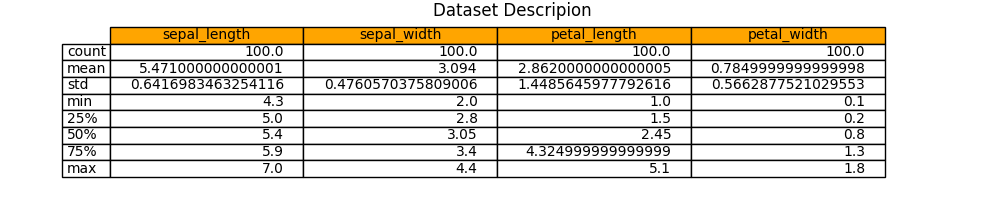
\includegraphics[scale=0.6]{desc_plot}
\caption{Dataset description after running df.describe()}
\centering
\end{figure}

\section{Workflow Analysis}
For the classification problem I compared four algorithms.
\subsection{K-Nearest Neighbor}
k-NN is a non-parametric  classification method, the output is a class membership. An object is classified by a plurality vote of its neighbors, with the object being assigned to the class most common among its k nearest neighbors (k is a positive integer, typically small). If k = 1, then the object is simply assigned to the class of that single nearest neighbor\cite{knn}
\subsection{Gaussian Bayes}
Gaussian Bayes classifier belongs to the Naive Bayes family that uses a simple technique for constructing classifiers: models that assign class labels to problem instances, represented as vectors of feature values, where the class labels are drawn from some finite set\cite{gbaye}
\subsection{Decision Tree}
Decision tree learning is one of the predictive modelling approaches used in statistics, data mining and machine learning. It uses a decision tree (as a predictive model) to go from observations about an item (represented in the branches) to conclusions about the item's target value (represented in the leaves).\cite{dec_tree}
\subsection{Local Feature Selection (LFS)}
Localized feature selection (LFS) is the third party classifier, it is a supervised machine learning approach for embedding localized feature selection in classification. The sample space is partitioned into overlapping regions, and subsets of features are selected that are optimal for classification within each local region. As the size and membership of the feature subsets can vary across regions, LFS is able to adapt to local variation across the entire sample space\cite{lfs}.
\section{Preprocessing Steps}
\subsection{Conversion to binary dataset}
The first preprocessing step was to convert our dataset from a multiclass dataset to a binary dataset. We selected only two kinds of species from the provided 3.
\begin{lstlisting}[language=Python]
clean_df = df.query('species =="setosa" or species=="versicolor"')
\end{lstlisting}
\begin{figure}[h]
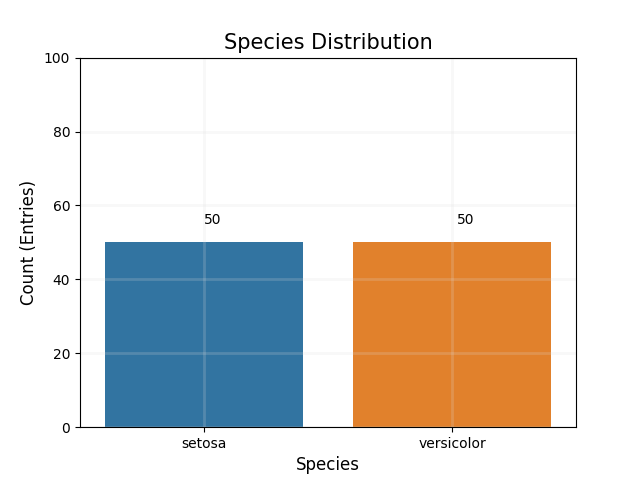
\includegraphics[scale=0.5]{classes}
\caption{Species Distribution}
\centering
\end{figure}
\clearpage
\subsection{Data splitting into training and test set}
I splitted the dataset into training and dataset with the ratio of 8:2. Below figure show the specie distribution when plot against Sepal Length and Width

\begin{figure}[h]
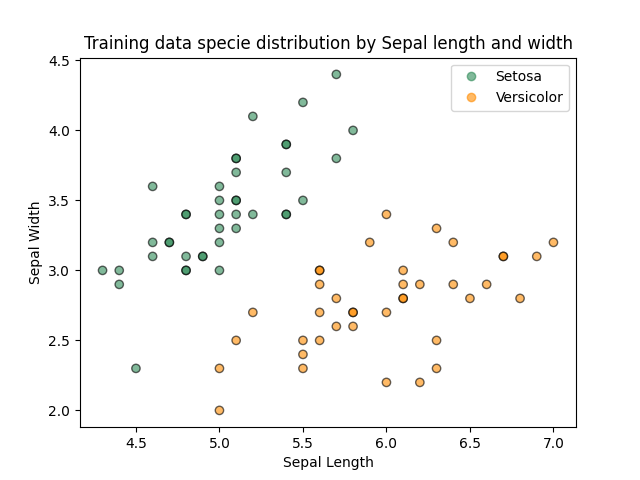
\includegraphics[height=5cm]{training}
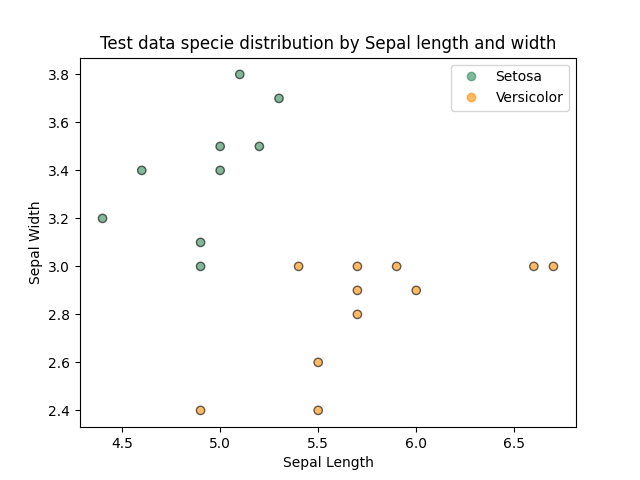
\includegraphics[height=5cm]{test}
\caption{Training an Test dataset}
\end{figure}
\section{Comparison}
Having been able to make the third party software work, I proceeded to the main problem which was to compare the performance of each classifier on our new binary dataset.

\begin{figure}[h]
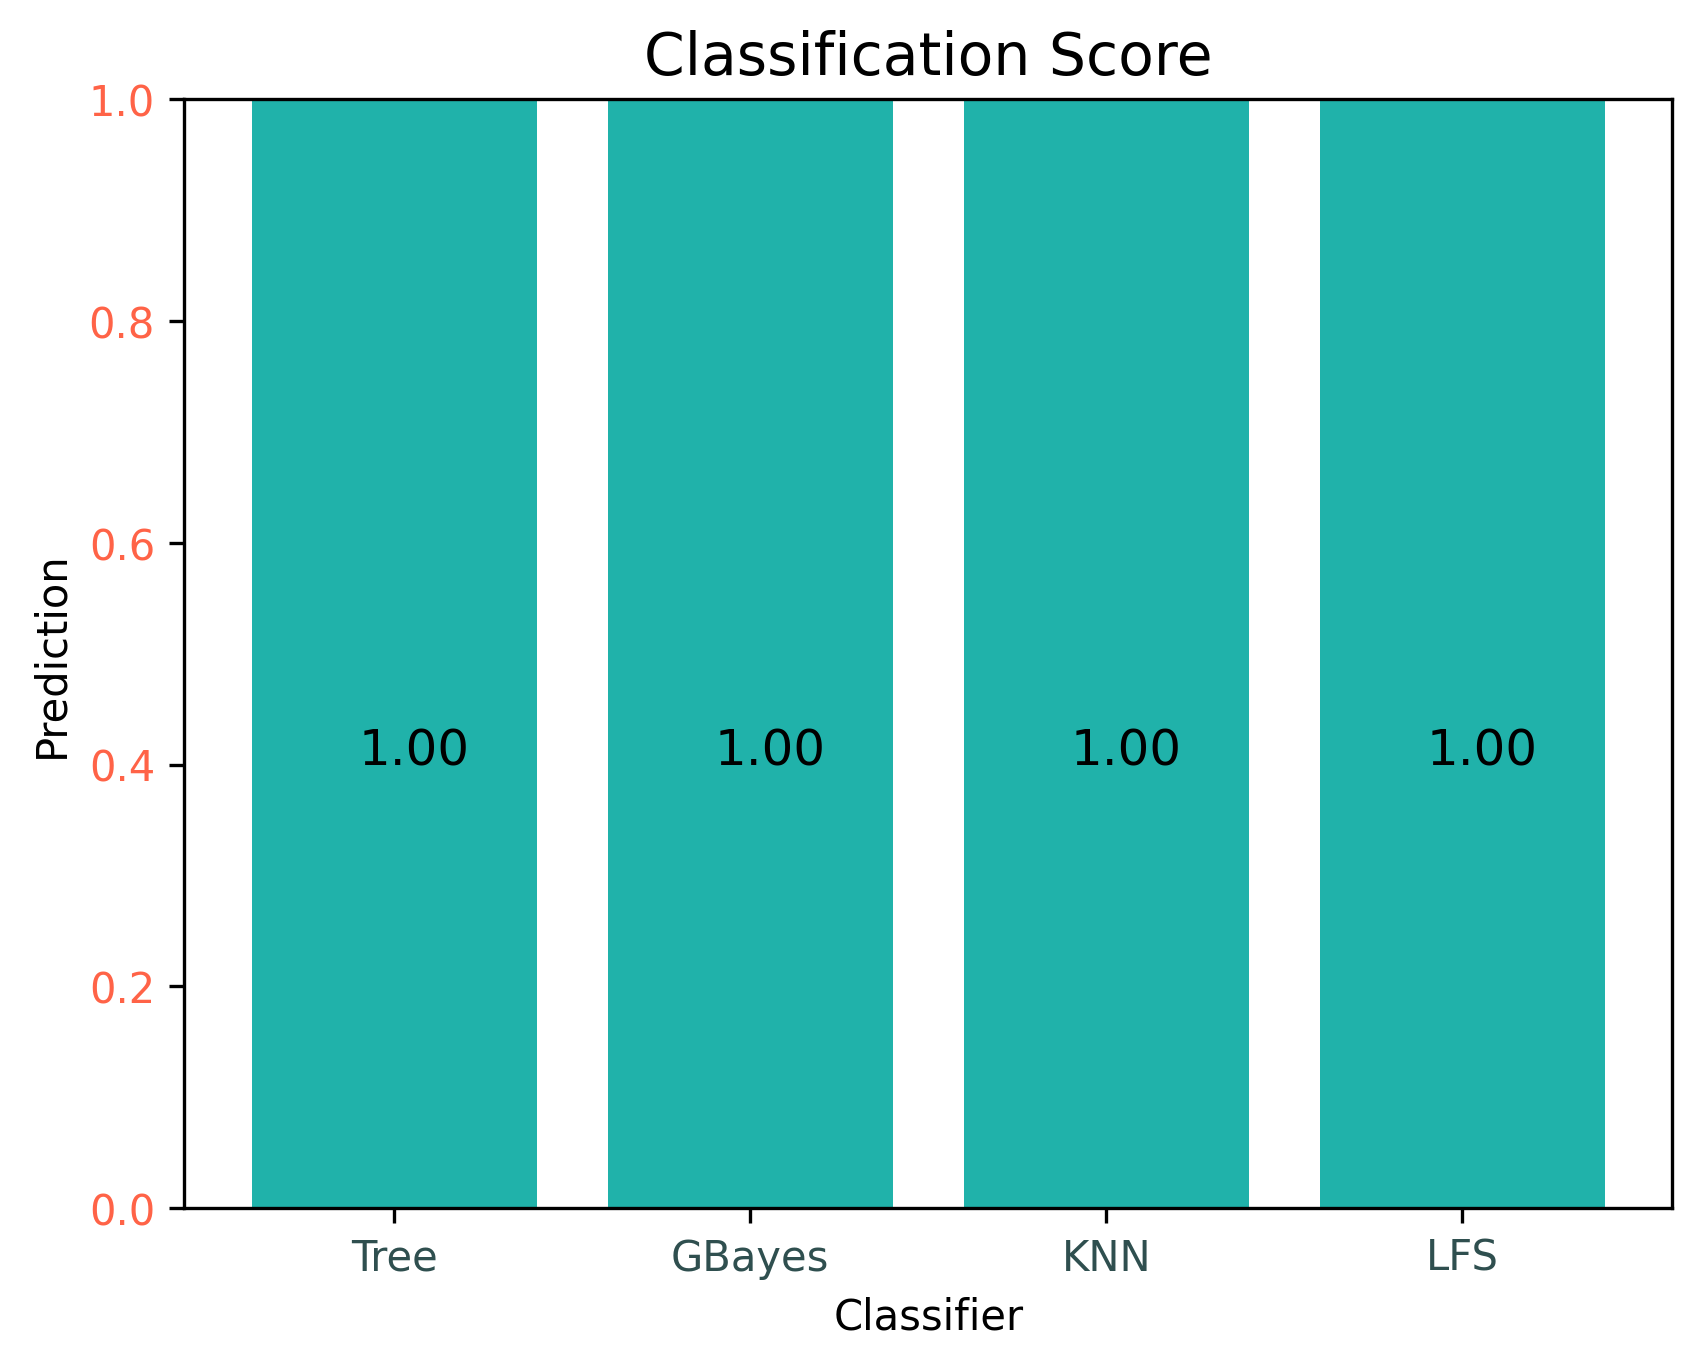
\includegraphics[scale=0.5]{classification_score}
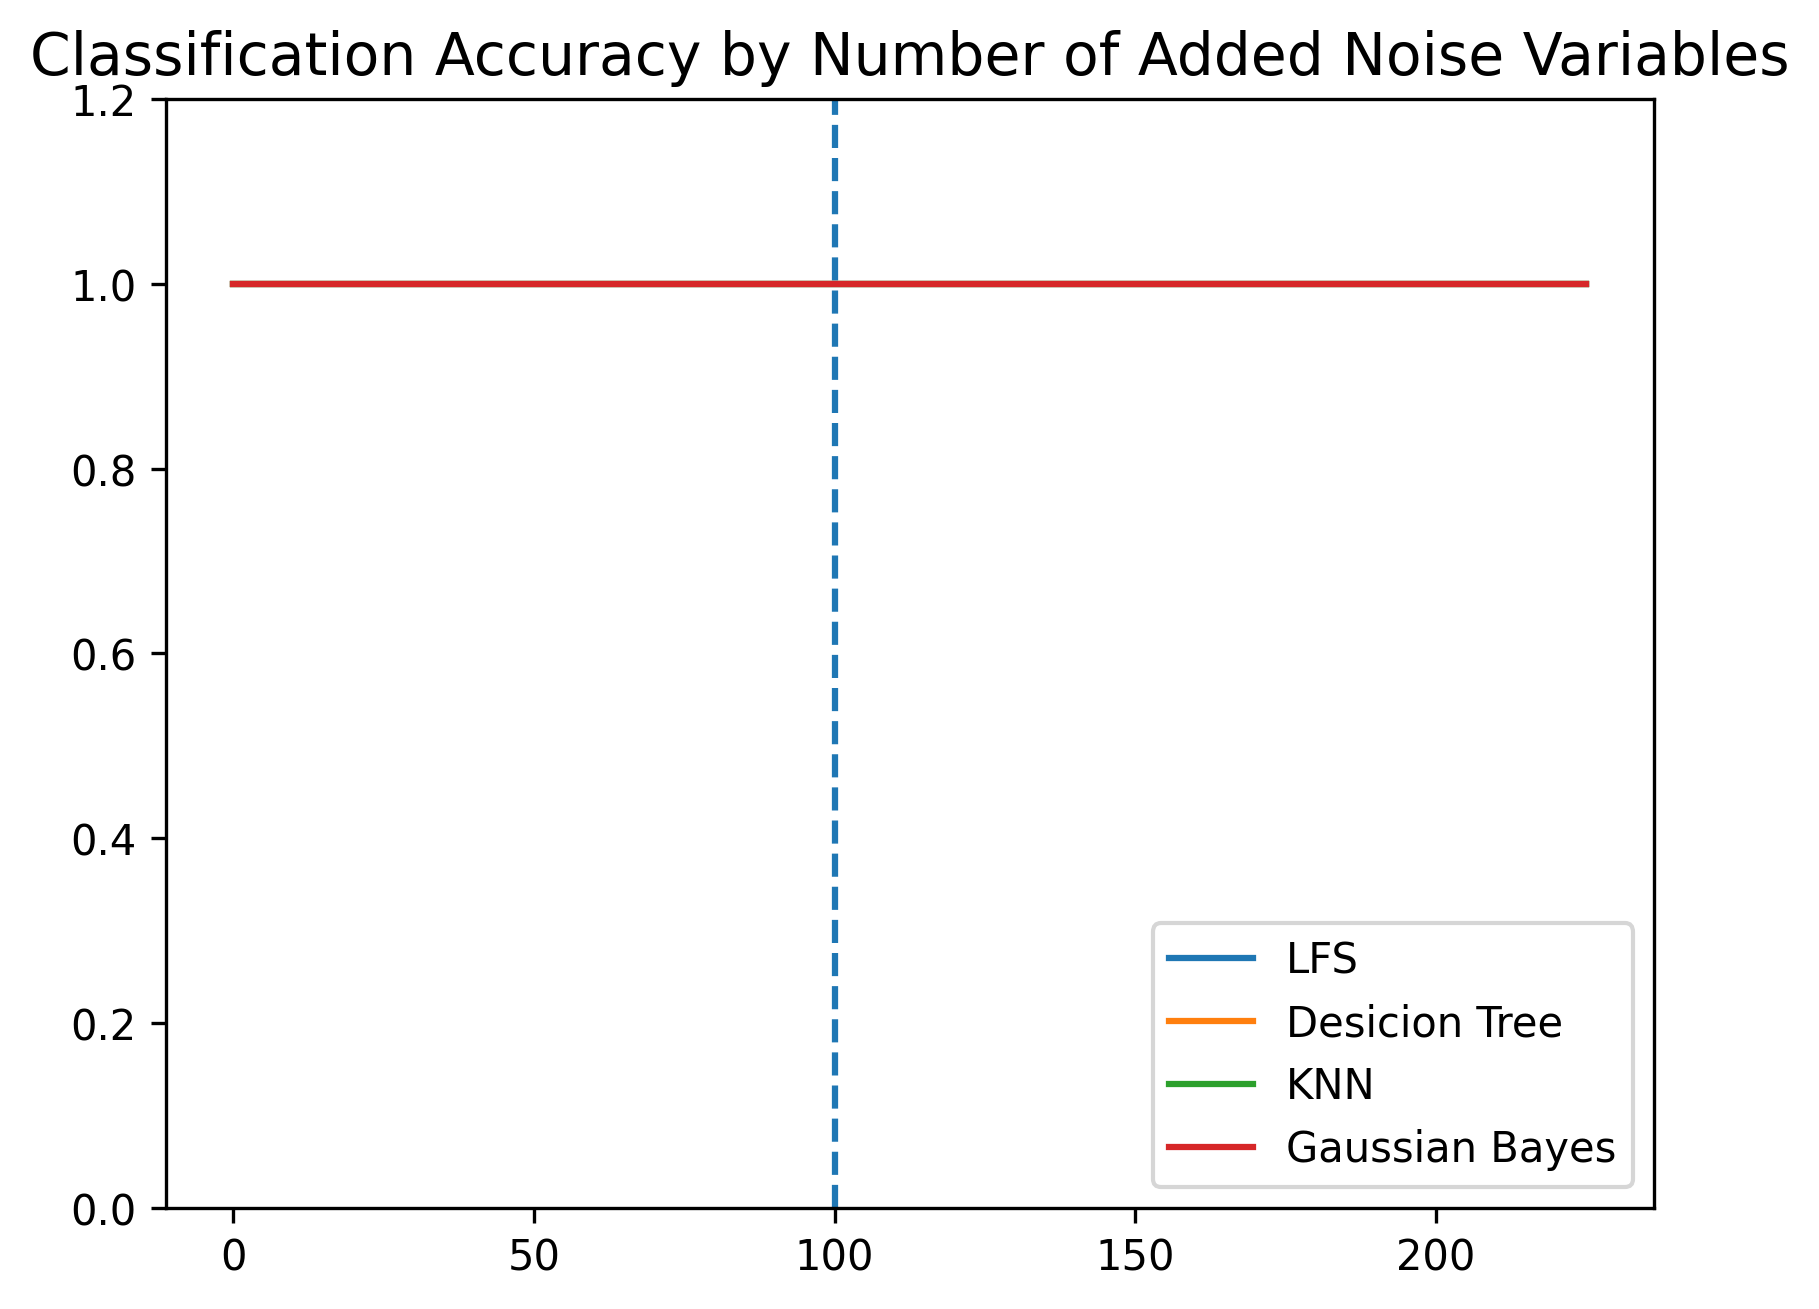
\includegraphics[scale=0.5]{classification_noise}
\caption{Comparison}
\end{figure}
The four classifiers performed brilliantly on the clean dataset. I went ahead to add noise to the dataset do another comparison.
Despite the introduction of noise the four classifiers perform equally well.
\section{Conclusion}
As much as LFS did perform well in this comparison, I noticed that it only works with certain dataset and can only perform binary classification. For such a promising package these limitations would negatively affect how far it could go.
\begin{thebibliography}{9}
\bibitem{lfs}
Dhindsa et al., (2020). LFSpy: A Python Implementation of Local Feature Selection for Data Classification with scikit-learn Compatibility. Journal of Open Source Software, 5(49), 1958, https://doi.org/10.21105/joss.01958

\bibitem{dec_tree}
@MISC{
title = {Decision tree learning},
howpublished={\url{https://en.wikipedia.org/wiki/Decision_tree_learning}}
}
\bibitem{gbaye}
@MISC{
title = {Naive Bayes classifier},
howpublished={\url{https://en.wikipedia.org/wiki/Naive_Bayes_classifier#Gaussian_na%C3%AFve_Bayes}}
}
\bibitem{knn}
@MISC{
title = {k-nearest neighbors algorithm},
howpublished={\url{https://en.wikipedia.org/wiki/K-nearest_neighbors_algorithm}}
}

\end{thebibliography}

\end{document}
